%%
%% licence       kaneton licence
%%
%% project       kaneton
%%
%% file          /home/buckman/kaneton/view/papers/assignments/k1.tex
%%
%% created       matthieu bucchianeri   [tue feb  7 11:49:38 2006]
%% updated       matthieu bucchianeri   [tue feb  7 11:49:41 2006]
%%

%
% k1
%

\section{k1}

\subsection{General description}

The \textbf{k1} project consists in the development of the bootloader.

This bootloader just relocates the stuff needed by the future kernel
execution.

The relocation is not really necessary but we wanted the students
to understand low-level programming and more especially programming
in a very strict environment with no fine-grain allocator provided.

Needless to  say, the  student will have  to install and  activate the
protected mode and the  virtual memory (students choosing ia32 without
paging will have to find an alternative to virtual memory).

So in this project, the student has to write the entire code of the
bootloader. The only requirement is to be compliant with the structure
passed to the kernel.

This structure called \textbf{t\_init} is defined in the
file: \textit{core/include/kaneton/init.h}.

The \textit{mem} and \textit{memsz} fields indicate the available physical
memory of the system.

The \textit{kcode} and \textit{kcodesz} fields indicate the location and
size of the kernel binary in main memory.

The \textit{init} and \textit{initsz} fields indicate the location and
size of this init structure in main memory.

The \textit{modules} and \textit{modulessz} fields indicate the
location of the area used to store the modules.

The modules area is composed of:

\begin{enumerate}
  \item
    The number of modules: \textit{nmodules}.
  \item
    An array of modules.
\end{enumerate}

Each module is composed of:

\begin{enumerate}
  \item
    A module structure \textit{t\_module} containing a name and size fields.
  \item
    The module's data: binary, text etc.. depending on the module nature.
  \item
    The module name terminated by a zero character.
\end{enumerate}

The \textit{nsegments}, \textit{segments} and \textit{segmentssz} fields
indicate the area location containing the segment array. This array
describes the core's pre-reserved segments.

The \textit{nregions}, \textit{regions} and \textit{regionssz} fields
indicate the area location containing the region array. This array
describes the segments to be mapped after the initialisation of the
core region manager.

Indeed, many segments will be needless so this array only specify the
fundamental segments to map.

The \textit{kstack} and \textit{kstacksz} fields indicate the kernel
stack area location.

The \textit{alloc} and \textit{allocsz} fields indicate the location
and size of the fine-grain allocator survey area. This area will be
used by the \textit{malloc()} suite functions to provide fine-grain
allocator while no segment neither region manager are initialised yet.

The  init  structure   also  contains  machine-dependent  fields,  the
\textit{gdt} and the \textit{page-directory} if needed.

The code provided must be located in the directory
\textit{core/bootloader/arch/[architecture]/}.

The students should use the system defines. Be aware that this project
must lead students to understand the project source organisation.

The student will have to build the init structure using the minimum
of memory, the goal of the game being to pack this structure.

%
% ia32
%

\subsection{IA-32 implementation}

The physical memory layout for the Intel architecture is the following:

\begin{figure}[h]
\centerline{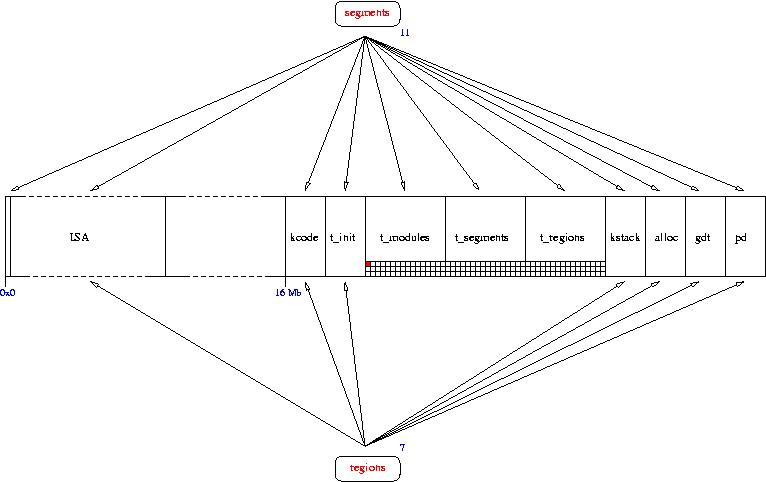
\includegraphics[scale=0.5]{figures/k1-memory-layout.jpg}}
\end{figure}

All the segments must be mapped at the kernel boot time.

Be careful to correctly initialise the machine-dependent fields
including \textit{gdt} and \textit{pd} which will be used by the microkernel
to retrieve the structures in main memory.

For this project,  you have to choose between using  paging or not. Be
careful:  once  this choice  done,  you  must  keep it  for  following
projects.

Here are the two possibilities:

\begin{itemize}
\item ia32-virtual, where you use paging
\item ia32-segment, without paging
\end{itemize}
